\chapter{Řídící elektronika}

Řídící elektronika osazovacího automatu má za úkol obstarávat následující funkce:
\begin{itemize}
\item komunikace s počítačem přes USB rozhraní
\item řízení motorů pro osy X, Y, Z, R (rotace)
\item řízení a měření vakua
\end{itemize}


Elektronika je založena na mikrokontroléru LPC1769 od firmy NXP. Je to moderní 32-bitový mikrokontrolér bežící na frekvenci 120 MHz s celou řadou integrovaných funkcí jako USB, ADC, DAC, UART a další. Jádrem mikrokontroléru je ARM\textregistered Cortex\textregistered-M3.

Mikrokontrolér komunikuje s řídícím SW přes USB rozhraní. Obstarává veškerou režii řízení krokových motorů a zároveň řídí všechny vstupně výstupní periferie. Blokový diagram je znázorněn na obrázku \ref{fig:ridici}, jednotlivé bloky jsou pak popsány v následujících podkapitolách.

\begin{figure}[h!]

  \centering
    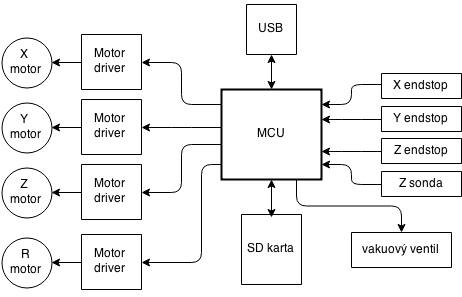
\includegraphics[width=0.8\linewidth]{obrazky/electronics.png}%
    \caption{Diagram řídící elektroniky.}
    \label{fig:ridici}
\end{figure}


\section{Firmware}

Firmware slouží jako mezičlánek mezi PC a hardwarem osazovacího automatu. Přijmá příkazy od řídícího SW a ty pak vykonává.

Ověřeným standardem pro instruování CNC strojů jsou tzv G-kódy. Programovací jazyk G, specifikován pod standardem RS274D umožňuje pomocí jednoduchých instrukcí řízení celého stroje. Bohužel standard RS274D ale není striktně dodržován a výrobci CNC strojů a řídících kontrolérů si upravují a vytváří vlastní specifické G-kódy.

Struktura G-kódu je následující: {\bf G}<číslo> <parametry>.\\
Pomocí {\bf G}<číslo> se rozlišuje o jaký příkaz se jedná a <parametry> jsou vstupní parametry příkazu. Jako ukázka poslouží kód na pohyb v osách {\bf G0}, ten bere parametry název osy a cílovou pozici osy.
\begin{verbatim}
  G0 X-10.3 Z12
\end{verbatim}

Parametry X-10.3 a Z12 tedy udávají, jaké osy a kam se mají pohnout. Není však specifikováno, jestli se jedná o absolutní, nebo relativní pohyb. K tomu slouží příkazy {\bf G90} (absolutní) a {\bf G91}(relativní) pohyb.
Všechny příkazy jsou vykonávány v posloupnosti tak, jak je mikrokontrolér obdrží. Následující posloupnost příkazů tedy nastaví stroj z počáteční pozice na pozici X0, Y10, Z0,4, poté provede relativní pohyb X5, Z2. Výsledná pozice stroje je tedy X5, Y12, Z0,4.

\begin{verbatim}
  G90
  G0 X0 Y10 Z=0.4
  G91
  G0 X5 Z2
\end{verbatim}

Obdobou G příkazů jsou M příkazy, které slouží na vykonávání příkazů přímo nesuvisejících s pohybem stroje. Pro příklad příkaz {\bf M42} slouží ke spínání vakuového ventilu.

Z důvodu komplexnosti celé diplomové práce by bylo napsání kvalitního firmware příliš časově náročné. Proto byl jako základ použit firmware Smoothie od autora Arthura Wolfa napsaný v programovacím jazyku C++. Pro uzpůsobení firmware pro osazovací automat bylo potřeba provést celou řadu úprav. Ne všechny požadované funkce byly totiž ve firmware dostupné. Chyběla hlavně podpora tlakového senzoru.
Zajímavou funkcí firmware je možnost jeho konfigurace přes textový soubor uložený na SD kartě. Ke každému pinu mikrokontroléru lze v konfiguračním souboru přiřadit libovolnou funkcu. 
Jako ukázka je uvedena konfigurace motoru k ose X. K pinu 0 na portu 2 mikrokontroléru byl přiřazen signál step (krok) motoru. Ovládání směru otáčení je na pinu 5 port 0, kde vykřičník znamená invertování směru otáčení. K portu 1 pinu 4 je nakonec přiřazen signál enable, který aktivuje motor.
\begin{verbatim}
  alpha_step_pin	2.0
  alpha_dir_pin		0.5!
  alpha_en_pin		1.4
\end{verbatim}


Protože firmware čte konfigurační soubor z SD karty, bylo zapotřebí ošetřit možnost zapnutí řídící elektroniky bez zasunute karty. Pokud by taková situace nastala, jednotlivé piny by byly v nedefinovaném stavu a mohlo by dojít k poškození osazovacího automatu. Proto byla ve firmware ke každnému použitému pinu přiřazena defaultní hodnota. Tato hodnota se dá později pomocí konfiguračního souboru změnit.
\\

Kompletní firmware s doprogramovanými funkcemi lze najít v příloze C. Jedná se již o zkompilovaný firmware ve formátu .bin  Z důvodu nadměrné velikosti nejsou zdrojové soubory součástí přílohy. Aktuální verzi zdrojových kódů modifikovaného firmware je ale možné získat přes internet za pomocí programu GIT příkazem:
\begin{verbatim}
  git clone https://github.com/Hyna/Smoothieware.git
\end{verbatim}
	




\section{Krokové motory a jejich drivery}

Horní a spodní kamera se připojuje přes USB rozhraní přímo do počítače nezávisle.

Jelikož je osazovací automat koncipován spíše na prototypovou výrobu, případně na první série DPS, není rychlost osazování kritická. I přesto byl ale kladen důraz na dosažení co největší osazovací rychlosti.

Jako vhodný typ motorů připadaly v úvahu krokové motory a servo motory. Servo motory by dozajista byly lepší volbou pro svůj velký kroutící moment a uzavřenou smyčku řízení. Oproti krokovým motorům jsou ale náročnější na řízení a mají vyšší cenu.
Volba tak padla na krokové motory u kterých je řízení jednodušší. Za použití driveru je lze ovládat jen pomocí signálu Krok a Směr (STEP a DIRECTION). Řízení je pak otevřenou smyčkou, krokový motor nemá žádnou zpětnou vazbu.

Může řídit jen jen zátěž, která je v rozsahun na kterou byl dimenzován. V opačném případě dochází ke ztrátě kroku a tím i pozice.

U krokového motoru se vzrůstající rychlostí rotace klesá kroutící moment. Od jakých otáček dochází k poklesu je ale zavislé na napájecím napětí. To je názorně vidět na momentové charakteristice pro motor SX17-1005LQEF od české firmy Microcon. Právě tento motor byl do konstrukce použit.


\begin{table}[h!]
  \caption{Katalogové parametry motoru SX17-1005LQEF }
  \begin{center}
  	\small
	  \begin{tabular}{|c|c|c|c|}
	    \hline
	    Statický moment [Nm]		& Příruba 		& Jmenovitý proud [A]	& Krok [°]	\\
	    \hline\hline

		0,51				& Nema 17		& 1,0			& 1.8		\\

	    \hline
	  \end{tabular}
  \end{center}
\end{table}

Konečná volba napájecího napětí byla dána s ohledem na vakuové ventily. Ty potřebují pro spolehlivý provoz napájení 24V, viz kapitola Vakuum. Celé zařízení tedy bude používat jednotné napájení 24V, aby odpadla nutnost mít dva různé napájecí zdroje.


Pro řízení motorů byl použit Pololu driver s integrovaným obvodem DRV8825 od Texas instruments. Driver je schpný bez aktivního chlazení do motoru dodávat až 1.5A při napájecím napětí do 45V. Plně tak vyhovuje pro použití s vybraným typem motoru SX17-1005. Navíc disponuje variabilně nastavitelným mikrokrokováním os 1/2 až do 1/32. 
Zvolený motor má krok 1.8° což odpovídá 200 krokům na otáčku. Na volbě mikrokroků tak bude záviset teoretická přesnost pozicování.

\begin{figure}[h!]

  \centering
    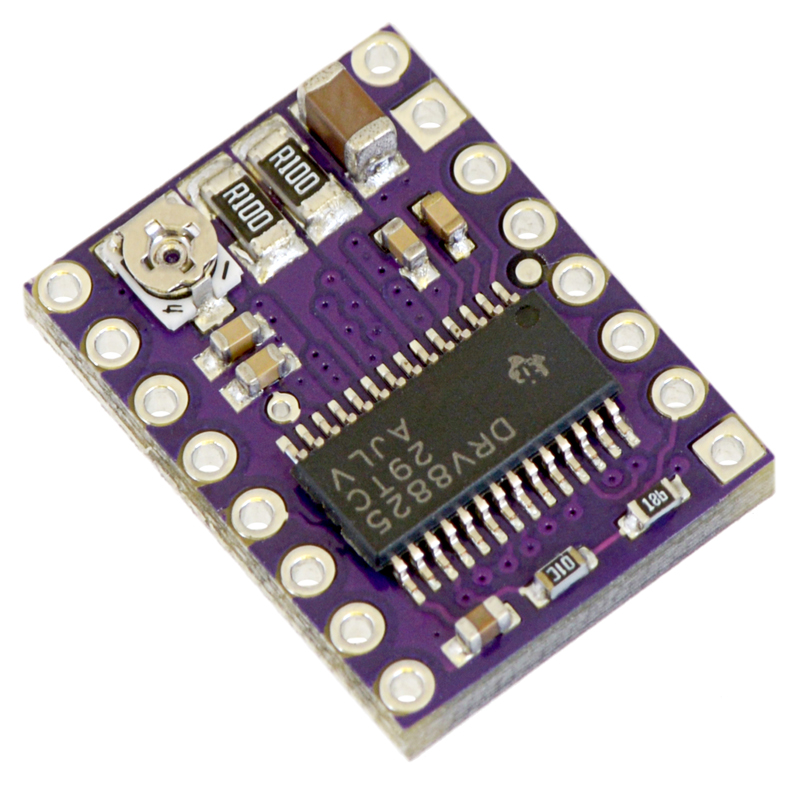
\includegraphics[width=0.4\linewidth]{obrazky/DRV8825.jpg}%
    \caption{DRV8825.}
\end{figure}

Jednoduchým výpočtem pak zjistíme, kolik kroků bude potřeba pro pohyb dané osy na jeden mm a teoretickou přesnost pozicování. Parametry kroky/mm je později použit na klaibraci os.
 
Použitý řemen GT2 má rozteč 2mm a řemenice má 20 zubů – viz kapitola o mechanické konstukci.
Krok na mm = (kroků na otáčku * mikrokroky) / (rozteč zubů řemenu  * počet zubů řemenice)
přesnost pozicování se pak vypočte jako převrácená hodnota počtu kroků na mm.

\begin{table}[h!]
  \caption{Mikrokrokování }
  \begin{center}
  	\small
	  \begin{tabular}{|c|c|c|}
	    \hline
	    Mikrokrokování		& Kroků na mm 		& Přestnost pozicování [um] 	\\
	    \hline\hline

		1 – celý krok 		& 5			& 200 				\\
		\hline
		1/2			& 10			& 100				\\
		\hline
		1/4			& 20			& 50				\\
		\hline
		1/8			& 40			& 25				\\
		\hline
		1/16			& 80			& 12,5				\\
		\hline
		1/32			& 160			& {\bf 6.25} 			\\
		\hline
	    \hline
	  \end{tabular}
  \end{center}
\end{table}

Jak vyplývá z tabulky, pro režim mikrokrokování 1/32 vychází teoretická přesnost 6,25 um. Co nejpřesnější pozicování je při osazování součástek žádoucí, proto byl driver nakonfigurován do tohoto režimu pomocí jumperů na konektoru MS4. Pro režim  1/32 se signály MS1, MS2 a MS3 připojují na Log 1.   Driver je ovládán signály EN – aktivace driveru, STEP - krok a DIR – směr přímo z procesoru. Konektor M4 pak slouží pro připojení krokového motoru. Význam a konfiguraci dalších pinů driveru lze najít v datasheetu.

\begin{figure}[h!]

  \centering
    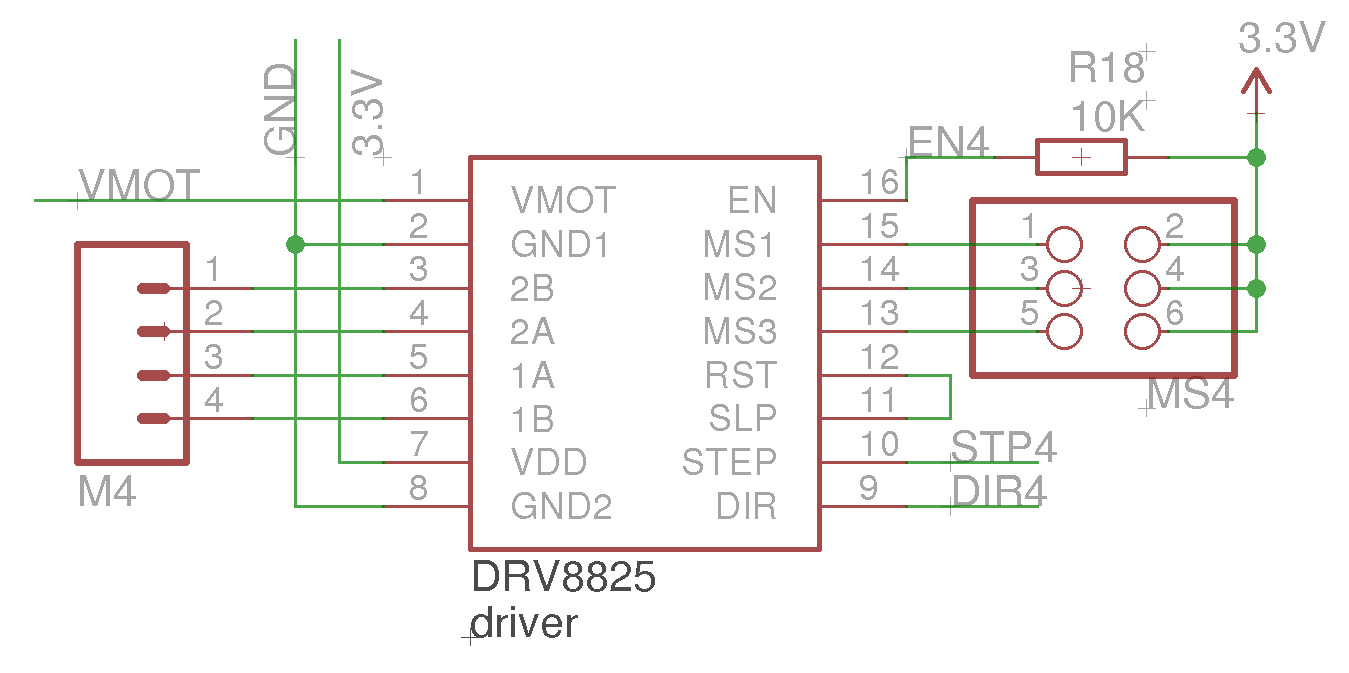
\includegraphics[width=0.8\linewidth]{obrazky/motorDriver.png}%
    \caption{DRV8825.}
\end{figure}

\begin{figure}[h!]

  \centering
    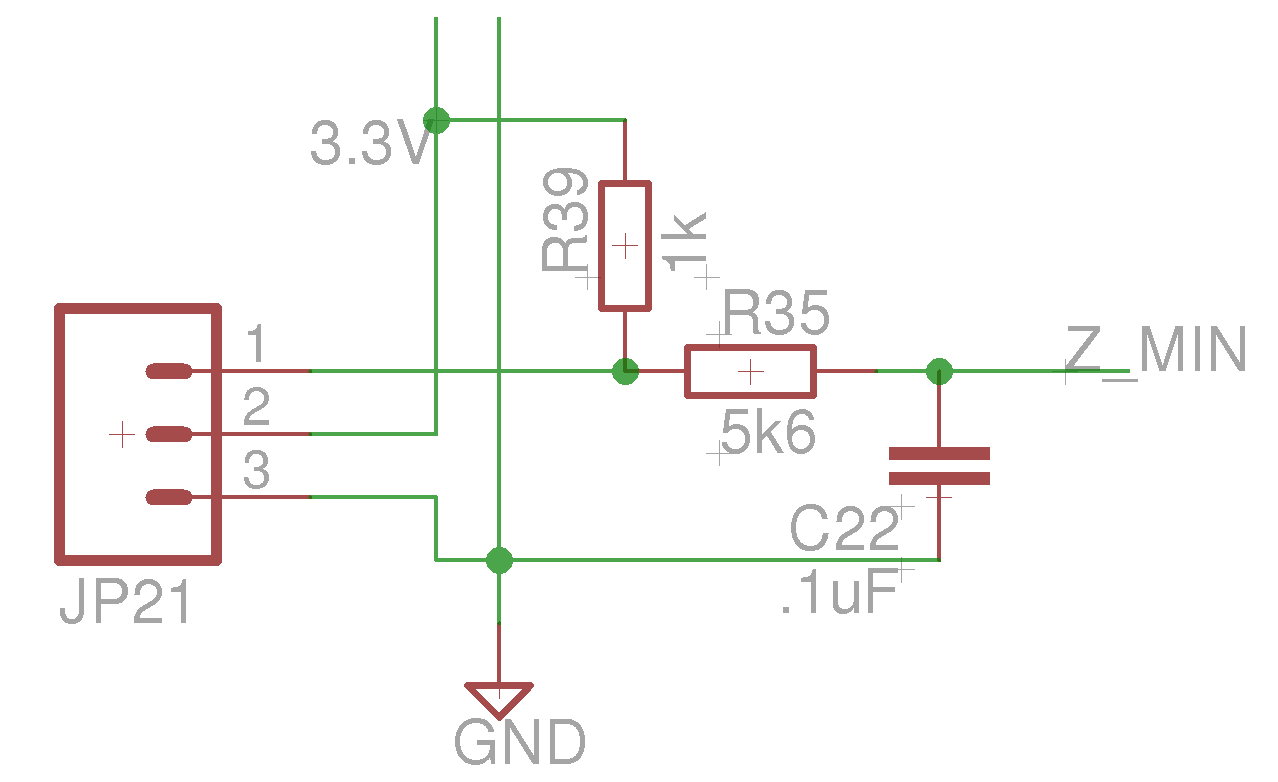
\includegraphics[width=0.6\linewidth]{obrazky/endstops.png}%
    \caption{Koncové dorazy.}
\end{figure}



\section{USB a elektromagnetická kompatibilita}

Mikrokontrolér disponuje nativní podporu USB protokolu verze 2.0, nebylo tak nutno žádných externích převodníků. Zapojení vychází z katalogového doporučení od výrobce mikrokontroléru. Odpory R8 a R9 na impedanční přizpůsobení, kondenzátory C4 a C5 na potlačení rušivých vysokofrekvenčních sgnálů.

\begin{figure}[h!]

  \centering
    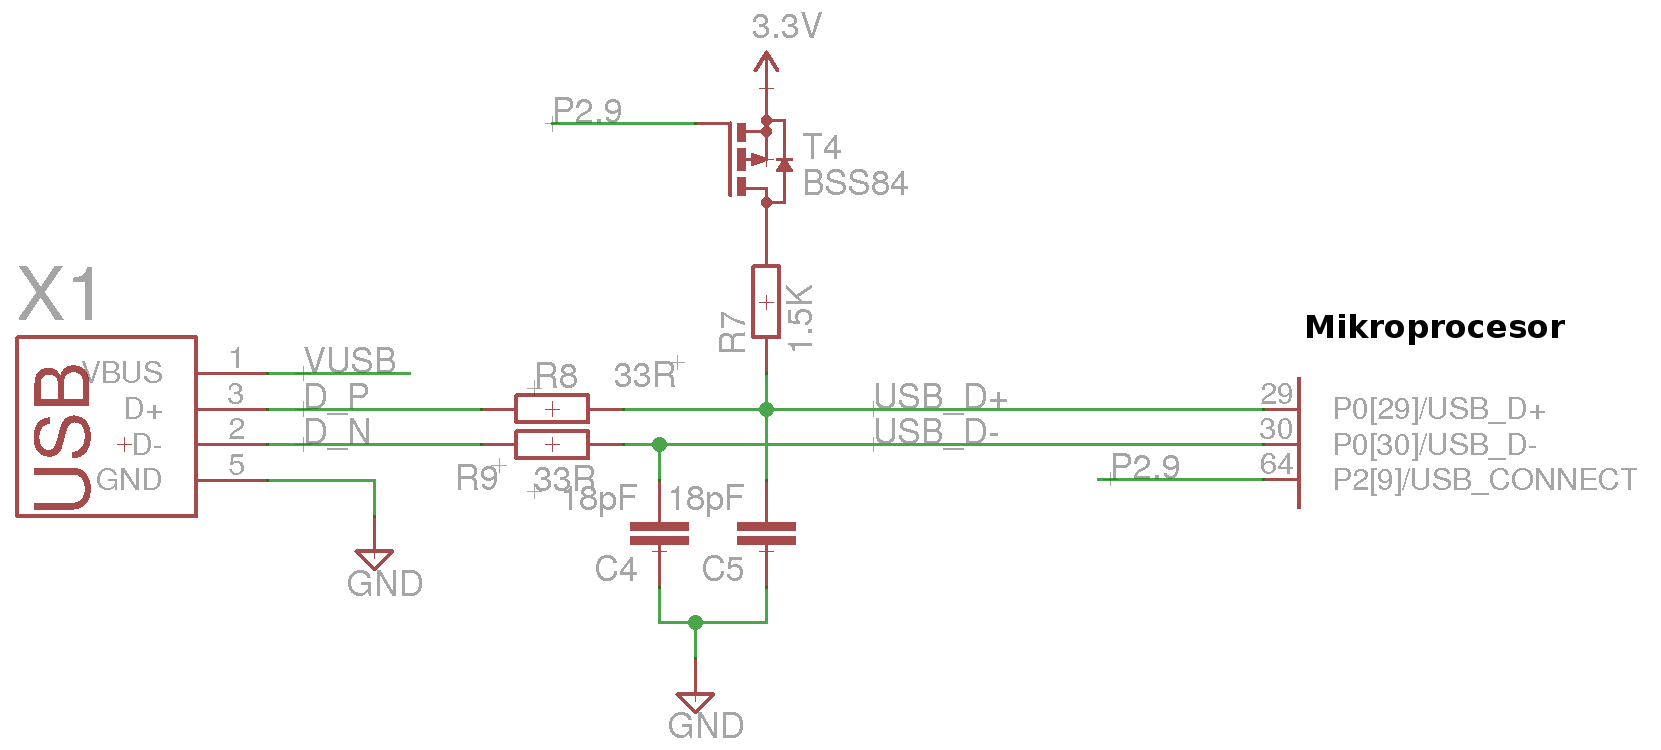
\includegraphics[width=0.8\linewidth]{obrazky/usb.png}%
    \caption{Zapojení USB.}
\end{figure}

Na následujícím obrázku je vidět původní zapojení prototypu řídící elektroniky. Jak bylo řečeno, vychází z doporučeného zapojení od výrobce a bylo navíc doplněno o kondenzátory C4 a C5 pro potlačení rušení dle \cite{intel}. V průběhu testování a psaní řídícího SW se ale bez zjevné příčiny stávalo, že došlo k přerušení komunikace s mikrokontrolérem. První podezření bylo na zamrzající (je to spisovný?) firmware mikrokontroléru a jeho reset. Pro ověření této doměnky byl k desce připojen externí převodník USB na sériové rozhraní. Po zamrznutí USB rozhraní se ale dalo stále připojit externím převodníkem a komunikovat s mikrokontrolérem. Problém tedy byl jen se samotným nativním USB rozhraním. 
První podezření na elektromagnetickou kmpatibilitu nastalo až při zapojování vakuové pumpy do rozvodné sítě. Deska reprodukovatelně přestávala komunikovat přes USB rozhraní. Měřením na osciloskopu se neprokázalo, že by se rušení šířilo vedením – napájecími kabely. 
Jednalo se tedy o rušení indukované. Za použití nacvakávacích feritů byl identifikován jako hlavní zdroj rušení USB kabel. Při používání feritů je důležité umisťovat je co nejblíže koncům kabelů.
Použitý propojovací USB kabel byl značky Goobay od Německého dodavatel a disponoval značkou CE. Rovněž použití jiných USB kabelů nepřinášelo bez feritu žádné zlepšení. 

\begin{itemize}
\item \verb|[ 19328.017144] hub 6-3:1.0: port 7 disabled by hub (EMI?), re-enabling...|
\item \verb|[ 19328.380201] usb 6-3.7: USB disconnect, address 4|
\end{itemize}





Pro potlačení elektromagnetické susceptibility byl obvod upraven do následující podoby.
Na signálových vodičích D+ a D- byl doplněn o tzv common mode filt 744232161 od WURTH ELEKTRONIK (USB signál je diferenciální). Rovněž signálová zem USB konektoru byla připojena přes ferit. Po této úpravě začal být obvod plně spolehlivý.

\begin{figure}[h!]

  \centering
    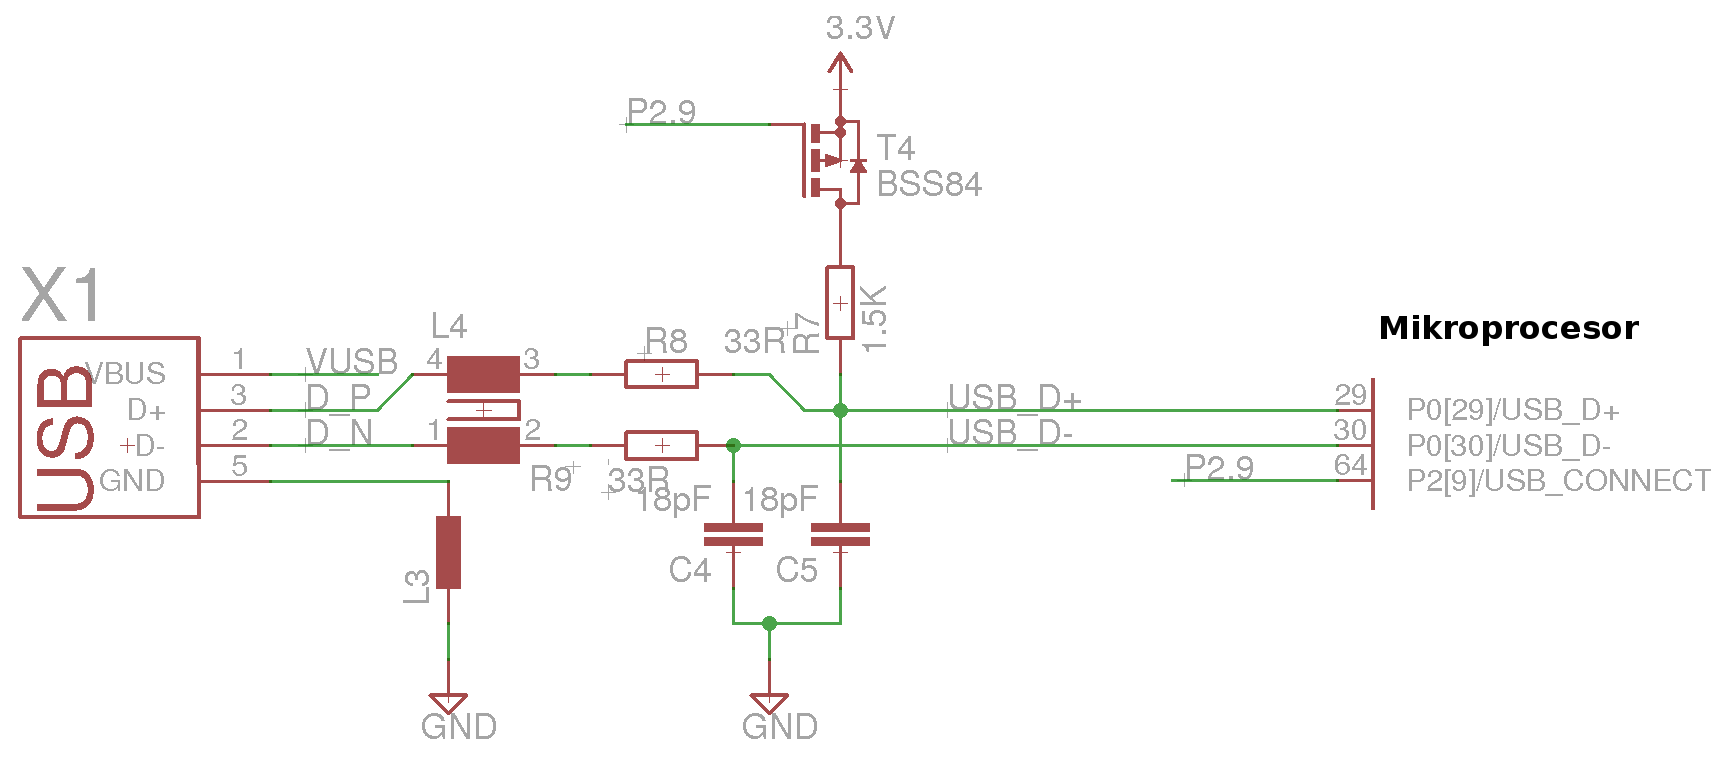
\includegraphics[width=0.8\linewidth]{obrazky/usbEMI.png}%
    \caption{Zapojení USB.}
\end{figure}

V této kapitole byly vyzdviženy jen nejdůležitější části obvodu, celé schéma zapojení je pak možé najít v příloze A

\section{Zapojení konektorů}

\begin{figure}[h!]

  \centering
    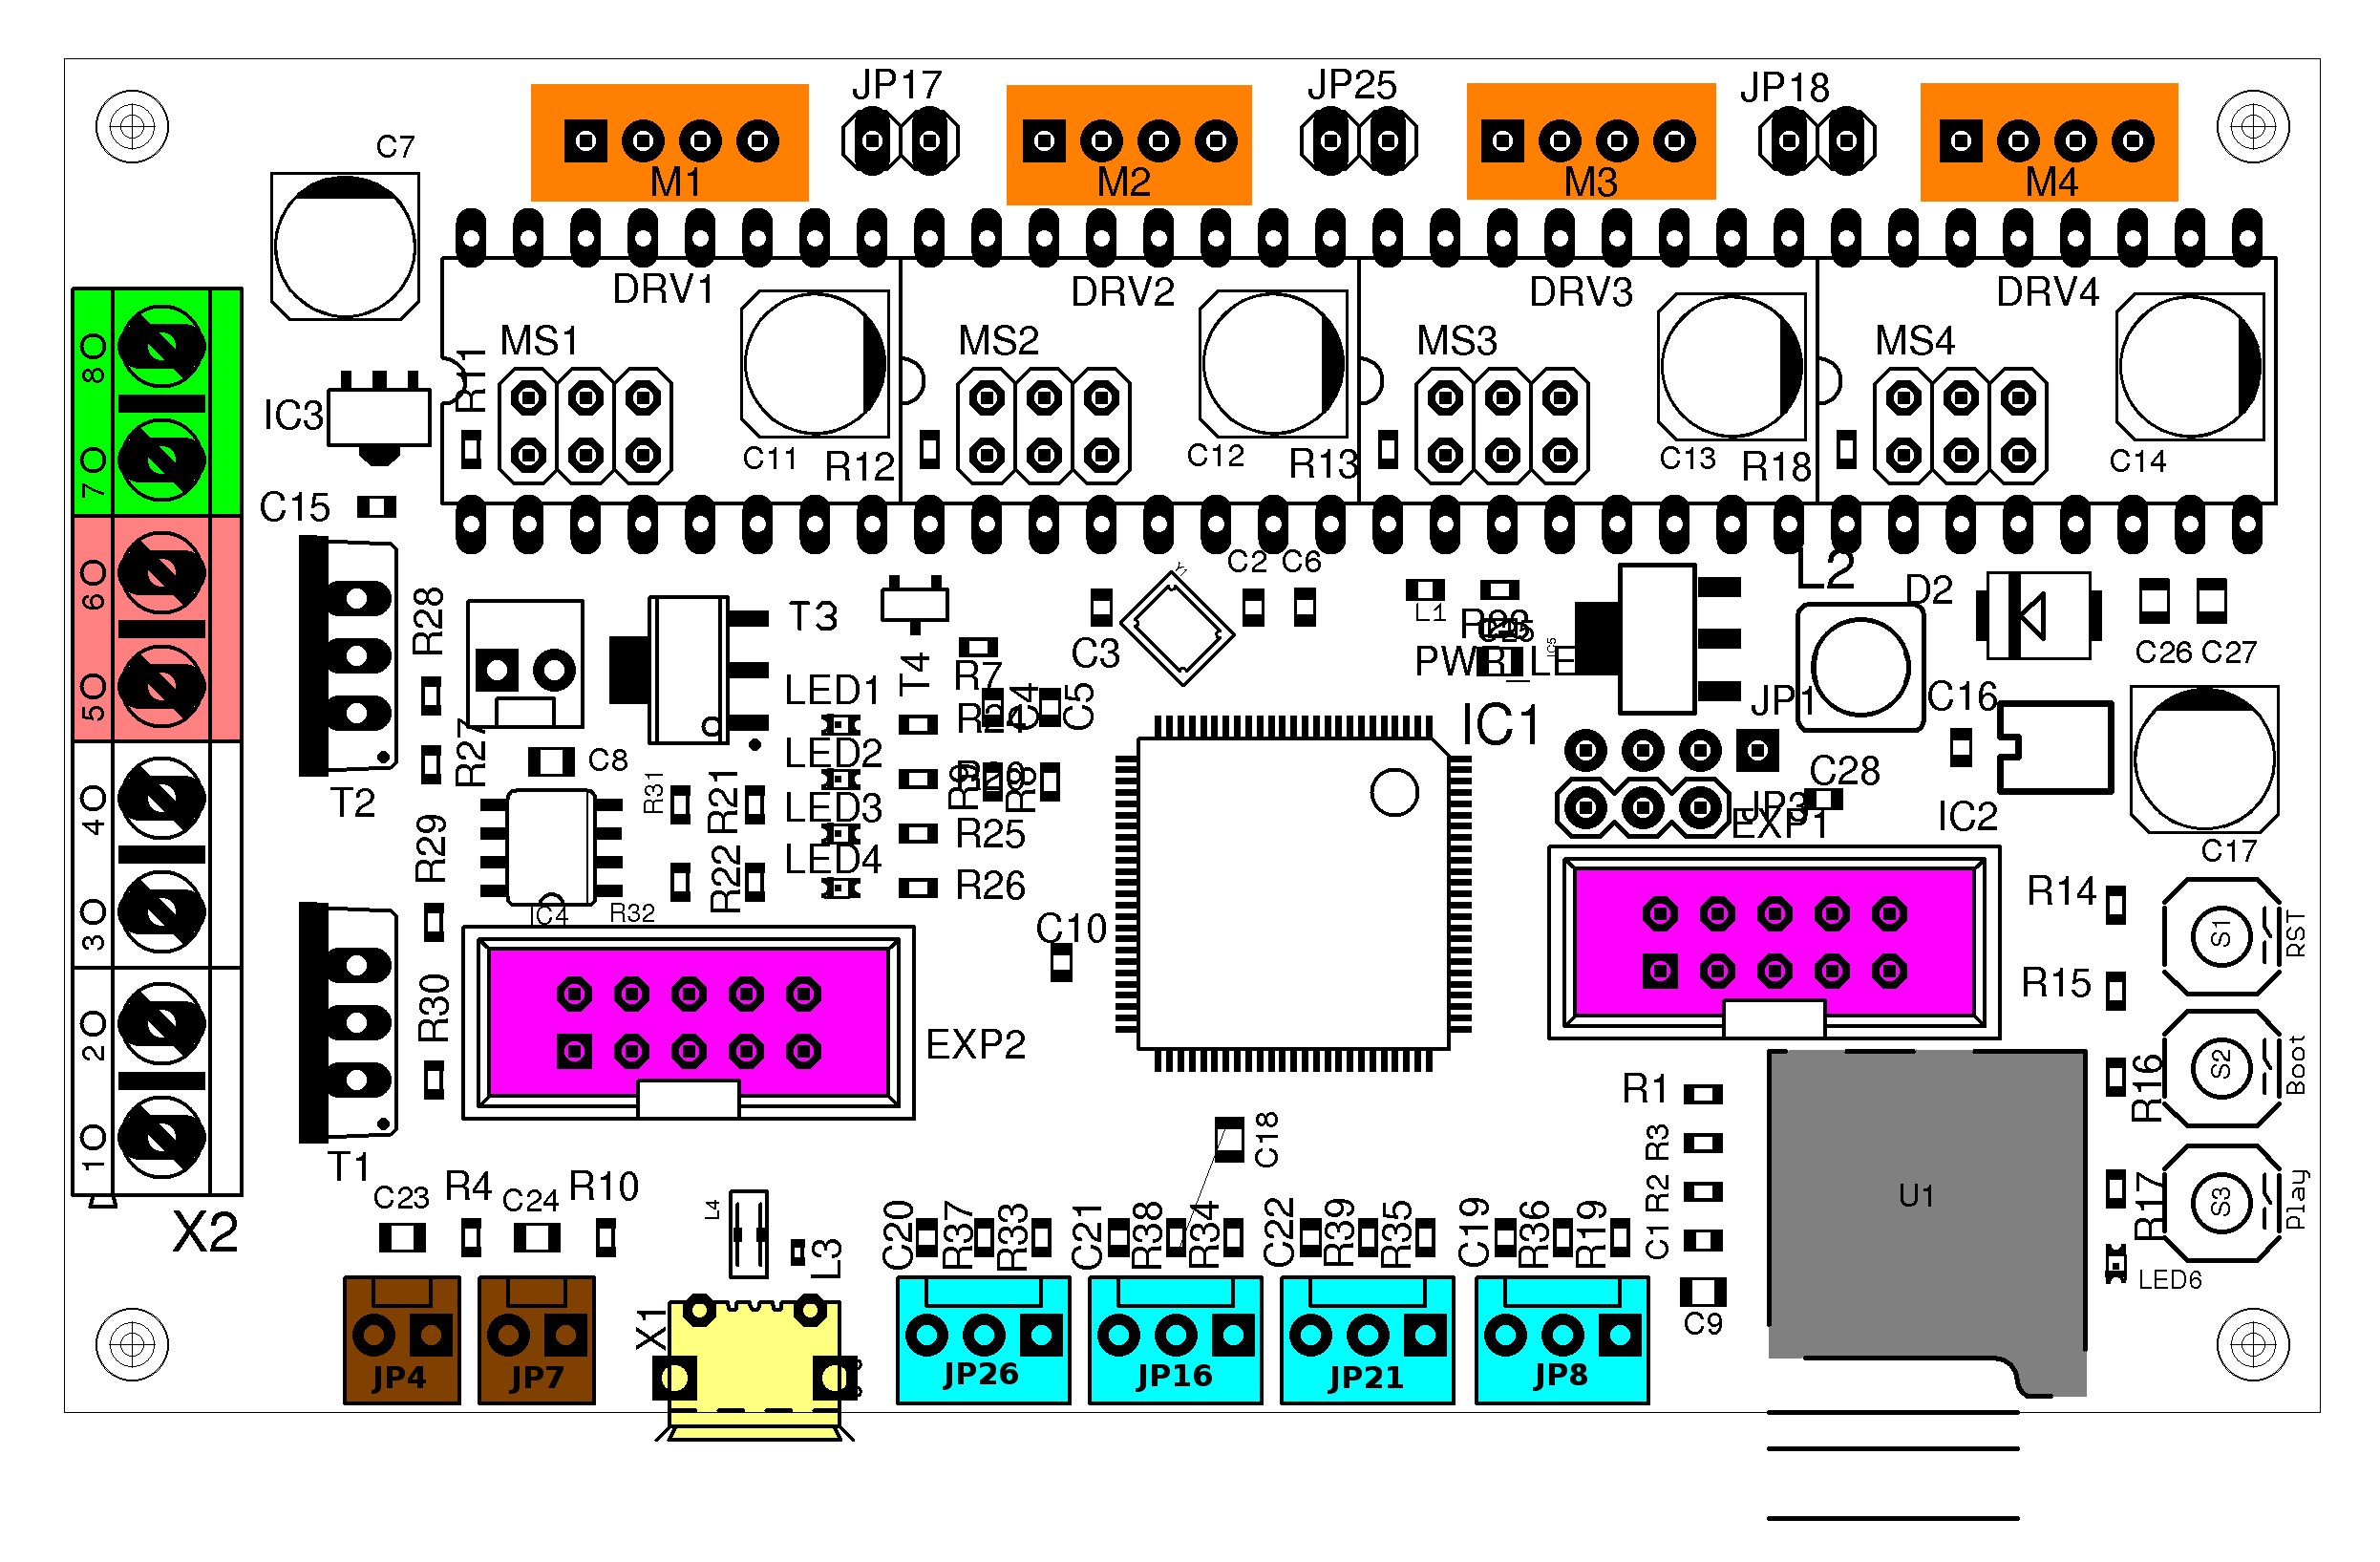
\includegraphics[width=0.8\linewidth]{obrazky/base3D_barva.png}%
    \caption{Zapojení konektorů.}
\end{figure}



\begin{table}[h!]
  \caption{Zapojení konektorů. }
  \begin{center}
  	\small
	  \begin{tabular}{|c|c|c|}
	    \hline
	    Barva			& Reference			& Význam  					\\
	    \hline\hline
		\cellcolor{blue!25}- 			& M1, M2, M3, M4		& Motory X, Y, Z a R				\\
		\hline
		-			& U1				& SD karta					\\
		\hline
		-			& X1				& USB konektor pro propojení s PC		\\
		\hline
		-			& X2-7, X2-8			& Napájení +24V					\\
		\hline
		-			& X2-5, X2-6			& Ventil pro řízení vakua			\\
		\hline
		-			& EXP1, EXP2			& Konektory pro připojení externího displaye	\\
		\hline
		-			& JP4, JP7			& ADC pro měření úrovně vakua 			\\
		\hline
	    \hline
	  \end{tabular}
  \end{center}
\end{table}

\begin{figure}[h!]

  \centering
    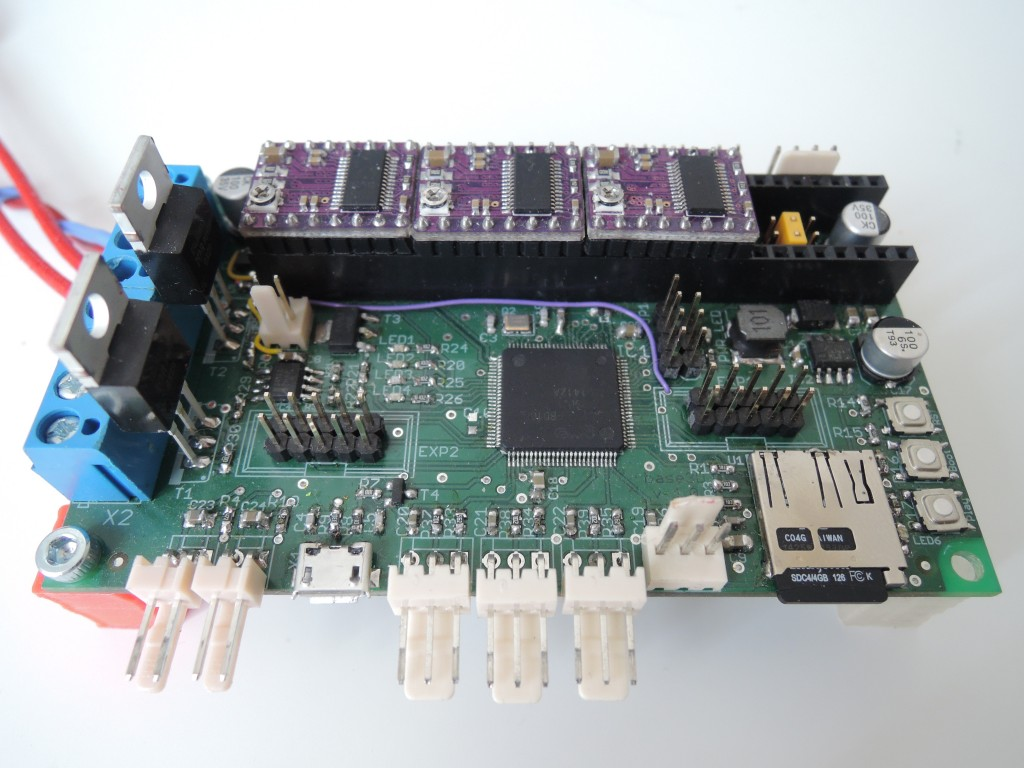
\includegraphics[width=0.8\linewidth]{obrazky/DSCN2185.JPG}%
    \caption{Osazená řídící elektronika ve verzi 1.0.}
\end{figure}


